Hoy en día,
%cada vez se realizan más y mejores investigaciones en el área de la robótica,
%tanto a nivel nacional como internacional.

La evolución de 
%las plataformas robóticas industriales desde sus principios ha sido vertiginosa.
%En poco mas de 30 años las investigaciones y desarrollos sobre robótica industrial,
%han permitido que los robots tomen posiciones en casi todas las áreas productivas y tipos de industria.

La manipulación de 
%dispositivos complejos ha dejado de ser una problemática sólo para las grandes
%empresas del rubro.
%El avance en las técnicas de la robótica y la difusión de la tecnología han dado como resultado,
%que la construcción de un dispositivo robótico,
%también sea un desafío para estudiantes e investigadores.

Las pocas soluciones existentes a la hora de implementar 
%interfaces de control,
%para este tipo de aparatos son de dos tipos:
%Aquellas que son propiedad de las empresas que fabrican las piezas de los dispositivos,
%y las que son implementadas por el propio equipo de desarrollo.
%En el primer caso,
%estas interfaces suelen ser muy restrictivas y poco flexibles;
%en el segundo caso,
%son muy rústicas y requieren la dedicación de recursos humanos y tiempo valioso para el equipo,
%que no se encuentra entre las metas del dispositivo en desarrollo.
%Todo esto limita el desarrollo de mejores aplicaciones y la experimentación con diferentes modelos.

Por otro lado, debido a todas las problemáticas actuales,
es fundamental 
%desarrollar una interfaz de control que las solucione,
%unificando las diferentes herramientas y optimice los recursos para la investigación de nuevas tecnologías.

A continuación, en la Figura 1, se señalan las fases por las cuales,
%cualquier investigador debe pasar,
%para poder probar una rutina determinada en una plataforma robótica:
%
%\begin{figure}[htp]
%	\begin{center}
%		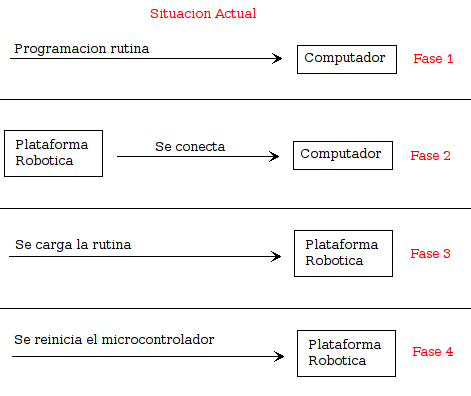
\includegraphics[scale=0.7]{img/user-sist}
%		\caption{Comunicación y perturbaciones}
%	\end{center}
%\end{figure}

\subsubsection{Identificación de problemas y deficiencias}
Debido a la situación anteriormente planteada,
se identificaron las siguientes problemáticas: 
\begin{itemize}
    \item 
\end{itemize}

\subsection{Caracterización del cambio}

\subsubsection{Características y potencialidades deseadas}
	Se espera que el sistema a desarrollar posea y/o sea capaz de:
%	\begin{itemize}
%		\item \textbf{Interfaz Gráfica de Usuario:}
%				
%		\item \textbf{:}
%
%		\item \textbf{Alta Modularidad:}
%			Con respecto a la construcción en sí del \emph{software},
%			se desea que ésta sea de carácter modular, para poder distribuir de manera más óptima,
%			las distintas funcionalidades que son necesarias para las plataformas robóticas que posee nuestro nicho 
%			de investigación, el Centro de Robótica de la UTFSM,
%			facilitando la implementación de funcionalidades futuras y compatibilidad con nuevos modelos del rubro.
%
%		\item \textbf{Portable a otros sistemas Operativos:}
%			Es necesario, no restringir una aplicación que busca suplir un problema tan importante en el área de la
%			robótica a un solo tipo de Sistema Operativo, por lo que se requiere utilizar herramientas que posibiliten
%			en el futuro poder portar la aplicación a diferentes plataformas computaciones (por ejemplo, Linux OS, Windows OS, etc)
%
%		\item \textbf{Estándar para el desarrollo de nuevos controladores, funcionalidades y aplicaciones:}
%			Además,
%			para que el sistema pueda seguir creciendo a diferentes y nuevos dispositivos,
%			es necesario que existan estándares para el desarrollo de nuevos componentes del sistema.
%
%		\item \textbf{Código Abierto:}
%			Para mantener la idea de que el sistema se pueda ampliar y desarrollar más allá de lo que dure nuestro proyecto,
%			es necesario que el mismo se rija bajo licencias que mantengan el código abierto a toda la comunidad.
%			Por ello,
%			éste se licenciará bajo la \emph{General Public Licence (GPL)}~\cite{GPL},
%			que resguarda y valida al proyecto en frente a la comunidad internacional.
%	\end{itemize}

La importancia de poder solucionar este tipo de problemas,
es que 
%el desarrollo en el área de la robótica en nuestro país,
%si bien es cierto, ha tenido variados avances, no está al nivel de países desarrollados
%que presentan las últimas vanguardias en el área.
%El desarrollo de Software es un tema clave a nivel de investigación en distintas áreas,
%pues potencia la calidad y ayuda a poder realizar investigaciones y desarrollos de una forma
%más expedita.

%Automatizando distintos procesos en el área de la investigación de la robótica,
%se está logrando que los especialistas que se desarrollan en éste ámbito,
%puedan no perder el tiempo con procedimientos que no tengan un gran significado,
%enfocándose sólo en aspectos mas importantes,
%dejando un poco de lado procesos de almacenamiento, tratamiento e interpretación de información.

% Conclusion
Por el hecho de que 
%en Chile existen distintos escenarios,
%donde prima la investigación en el área de la robótica,
%se está enfrentando una problemática latente.

El problema es complejo,
%tanto que existen varias empresas que encuentran rentable
%el desarrollo de software en esta área.
